\documentclass[compress]{beamer}

\usepackage[utf8]{inputenc}
\usepackage[T1]{fontenc}
\usepackage[french]{babel}
\usetheme{Amsterdam}

\usepackage{multicol}
\usepackage{listings}
\usepackage{color}

\usepackage{tikz}
\usetikzlibrary{shapes,arrows}

\lstset{language=caml, frame=single, basicstyle=\ttfamily\scriptsize, commentstyle=\color{dkgreen}}

\newcommand{\email}[0]{francois.ripault@epita.fr}

\definecolor{dkgreen}{rgb}{0,0.6,0}

\defbeamertemplate*{title page}{customized}[1][]
{
  \begin{center}
  \usebeamerfont{title}\inserttitle\par
    \usebeamerfont{subtitle}\usebeamercolor[fg]{subtitle}\insertsubtitle\par
    \bigskip
    \usebeamerfont{author}\insertauthor\par
    \scriptsize \texttt{\email} \par
    \usebeamerfont{institute}\insertinstitute\par
    \usebeamerfont{date}\insertdate\par
    \vfill
    \begin{figure}[h]
      \begin{tabular}{ccccc}
        
\includegraphics[scale=0.4]{../data/inria.jpg} & &
        
\includegraphics[scale=0.6]{../data/pps.png} & &
        
\includegraphics[scale=0.4]{../data/epita.jpg}
      \end{tabular}
    \end{figure}
    %\usebeamercolor[fg]{titlegraphic}\inserttitlegraphic
    \end{center} }

\newenvironment{tframe}[1]{
  \subsection{#1}
  \begin{frame}{#1}
  }{
  \end{frame}
  }

%% FIXME: title
\title{Soutenance de stage de fin de tronc commun : \\ Refonte du logiciel Coqdoc}

\author{François Ripault}

\begin{document}
\begin{frame}
  \titlepage
\end{frame}

\begin{frame}{Introduction}
  \begin{itemize}
    \item Stage effectué du 3 septembre 2012 au 11 janvier 2013
    \item Au sein de l'INRIA
    \item Refonte du logiciel de documentation Coqdoc
  \end{itemize}
\end{frame}
  \begin{frame}{Motivations du stage}
  \begin{columns}[2]
    \begin{column}{0.5\textwidth}
    Aspect ingénierie :
  \begin{itemize}
    \item Validation des acquis
    \item Acquisition de nouvelles compétences
    \item Production d'un logiciel
  \end{itemize}
    \end{column}
    \begin{column}{0.5\textwidth}
      Aspect recherche :
  \begin{itemize}
    \item Introduction aux sujets de recherche
      de PPS
    \item Interaction avec des scientifiques
  \end{itemize}
    \end{column}
  \end{columns}
\end{frame}

\begin{frame}
\tableofcontents
\end{frame}

\section{Présentation de l'entreprise}
\begin{tframe}{L'INRIA}
  Présentation de l'entreprise :
  \begin{itemize}
    \item Institut national de recherche en informatique et en automatique
    \item Activité scientifique centrée sur l'informatique, et ses interactions
      avec d'autres sciences.
    \item Collaborations avec de nombreux partenaires industriels et académiques
    \item Créateur de start-ups
  \end{itemize}
  \begin{figure}
        
\includegraphics[scale=0.4]{../data/inria.jpg}
  \end{figure}
\end{tframe}
\begin{tframe}{Le laboratoire PPS}
  Présentation du service
  \begin{itemize}
    \item Laboratoire Preuves, Programmes et Systèmes
    \item Équipe multi-disciplinaire
    \item Liens entre les mathématiques et l'informatique
  \end{itemize}

  \medskip

  Le Projet Coq
  \begin{itemize}
    \item Assistant de preuves
    \item Certifications de programmes, validation de preuves, recherche
      fondamentale en informatique
    \item Possède un logiciel de documentation : Coqdoc
  \end{itemize}
  \begin{figure}
        
\includegraphics[scale=0.6]{../data/pps.png}
  \end{figure}
\end{tframe}

\section{Le déroulement du stage}

\begin{tframe}{Objectifs de ce stage}
  \begin{block}{Objectif Principal : refaire Coqdoc}
    \begin{itemize}
      \item Être rétro-compatible
      \item Avoir une architecture extensible et simple
      \item Mieux intégrer le nouveau logiciel
    \end{itemize}
  \end{block}
  \begin{block}{Objectif secondaire : étendre le logiciel}
    \begin{itemize}
      \item Proposer de nouveaux contextes d'utilisation
      \item Exemple : Coq-Tex
    \end{itemize}
  \end{block}
\end{tframe}

\begin{tframe}{Fonctionnement de Coqdoc}
  \begin{figure}
    \lstinputlisting{input.v}
  \end{figure}
\end{tframe}

\begin{tframe}{Architecture du logiciel}
  \begin{figure}
    \begin{figure}
  \begin{tikzpicture}

  \node[draw, ellipse, thick, fill=blue!20] (V) at (-3,0) {Coq File};
  \node[draw, ellipse, thick, fill=blue!20] (Tex) at (-3,-1) {Coq-tex File};

  \node[draw, thick, fill=blue!20] (front) at (1,-0.5) {Front-end};
  \draw[->] (V.east) -- (front.west);
  \draw[->] (Tex.east) -- (front.west);

  \node[draw, thick, fill=blue!20] (eval) at (1, -2) {Evaluation};
  \draw[->, -latex'] (front.south) -- node[right, color=black] {AST} (eval.north);

  \node[draw, thick, fill=red!20] (coqtop) at (5,-2) {Coqtop};
  %\draw[->, dashed, -latex'] (eval.east)  -- node[above, color=black] {Interaction} (coqtop.west);
  \draw[<->, dashed] (eval.east)  -- node[above] {Interaction} (coqtop.west);

  \node[draw, thick, fill=blue!20] (back) at (1, -4) {Back-end};
  \draw[->] (eval.south) -- (back.north);

  \node[draw, thick, fill=yellow!20] (spec-html) at (-3, -3.5) {Html spec};
  \draw[->,-latex'] (spec-html.east) -- node[above] {Specification} (back.west);
  \node[draw, thick, fill=yellow!20] (spec-latex) at (-3, -4.5) {LaTeX spec};
  \draw[->] (spec-latex.east) -- (back.west);

  \node[draw, thick, ellipse, fill=blue!20] (output) at (5, -4.5) {Output file(s)};
  \draw[->,-latex'] (back.east) -- node[above] {Print} (output.west);

  \end{tikzpicture}
\end{figure}

  \end{figure}
\end{tframe}

\begin{tframe}{Exemple de document de sortie}
\begin{center}
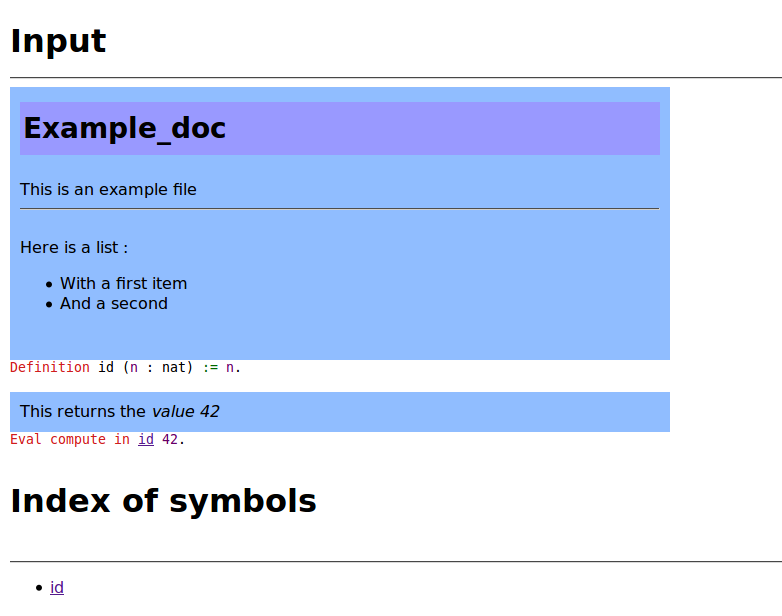
\includegraphics[scale=0.4]{input.png}
\end{center}
\end{tframe}

\begin{tframe}{Réalisation du stage}
  \begin{block}{Refonte de Coqdoc}
    \begin{itemize}
  \item Objectif partiellement accompli
  \item Le coeur logique du logiciel est implémenté
  \item Travail de finalisation restant à faire
  \item Bonne intégration de ce logiciel : réutilisation de l'existant
\end{itemize}
  \end{block}
  \begin{block}{Extension de Coqdoc}
    \begin{itemize}
      \item Le logiciel est facilement extensible
      \item Un prototype d'extension implémenté, pas encore intégré
    \end{itemize}
  \end{block}
\end{tframe}

\begin{frame}{Aspect recherche}
    \begin{itemize}
      \item Interaction riche avec les membres de l'équipe
      \item Groupe de travails sur Coq et sur la théorie de la réalisabilité
      \item Un jour de la semaine dédié à la recherche
      \item Présentation en anglais du logiciel (14 février) au groupe de travail
        Coq
    \end{itemize}
\end{frame}

\begin{frame}{Conclusion}
  \begin{itemize}
    \item Stage enrichissant
    \item Sujet très lié à l'aspect ingénierie
    \item Fortement ancré dans le monde de la recherche
  \end{itemize}
    \vfill
  \begin{center} \large Questions ? \end{center}
\end{frame}
\end{document}
